\openingarticle
\def\ppages{\pagerange{Norman:firstpage}{Norman:lastpage}}
\def\shorttitle{Re-assessing the Location of the Homeric Underworld in the Odyssey Book XI}
\def\maintitle{Re-assessing the Location of the Homeric Underworld in the Odyssey Book XI}
\def\shortauthor{Bertie Norman}
\def\authormail{jbn3@kent.ac.uk}
\def\affiliation{University of Kent}
\def\thanknote{\footnote{Bertie Norman started studying BA Ancient History at the University of Kent in 2014. His interests are focused on the euhemerist interpretation of mythology, which considers that myths and legends tell of past historical events. He specialises in archaeological analysis, reading Ancient Greek and Egyptian hieroglyphs. His previous interest has been the learning and deciphering of Ancient Hebrew, Aramaic, Canaan and Ugaritic scripts. He has a particular interest in comparative mythology, comparing Greek myths with those of Near Eastern cultures to gain a broader understanding of the undocumented relationships between Archaic Greek and other cultures.}}
%--------------------------------------------------------------
\mychapter{\maintitle}
\begin{center}
	{\Large\scshape\shortauthor \thanknote}\\[1em]
	\email \\
	\affiliation
\end{center}
\vspace{3em}
\midarticle
%--------------------------------------------------------------
\label{Norman:firstpage}
%----------------------------------------------------------------------------------------
	\begin{myabstract}
Homeric \marginnote{Abstract\\(in German see below)}poetry displayed the first basic structures of the Greek underworld: the encircling deep river of Oceans, the rivers of Styx, Acheron, Cocytus and the “dank house of Hades”. The aim of this article is to gain a general understanding of where Homeric underworld was located, specifically the underworld in The Odyssey Book XI. To explore the exact location itself, this article will use a combination of archaeological evidence, comparative linguistic analysis of Hittite and Egyptian stelai and papyri, and literary analysis of Homeric poetry.

\keywords[Keywords]{Homer, mythological geography, Odyssey, Hittite, Underworld, Book of the Dead, Cimmerians, Bronze Age Mediterranean.}
	\end{myabstract}
	
	
\lettrine[nindent=0em,lines=3]{T}{he}  purpose of this article is to understand the location of the Homeric Underworld, the Cimmerians in the \emph{Odyssey}, through the inspection of offerings. In this, Odysseus’ offerings at this area and their functions shall be compared with those mentioned in Hittite and Egyptian hymns, rituals and \emph{stelai}. Through translation, the analysis of Homer’s description of the Cimmerian location will challenge the suggestion (presented by Herodotus) that the area was in Scythia, (Hdt. Hist.4.1.2) and instead examine whether the Homeric location resides in Anatolia or Egyptian territory. As \textcite[356]{Morford2011} explains: “\emph{the geography of the Homeric Underworld is vague… Particularly in the precision that is evident in subsequent literature}”. Homer was the first known person to write about the structure of the Greek Underworld (influencing Plato and Virgil’s later works), so exploring where Homer considered the underworld to be will give a stronger understanding of Homeric geography and the impact it had on his successors’ writings.
	
	In the ‘East Face of Helicon’, \textcite[12]{West1997} demonstrated that the formation of the Ancient Greek language came from surrounding Mediterranean cultures in Asia Minor, the Levant and Egypt. His philological inspection leads one to wonder whether Greek rituals were influenced by the same foreign cultures that helped form the archaic Greek language. In his inspection of the chthonic myths in the \emph{Odyssey}, \textcite[425]{West1997} makes consistent comparisons between Greek and Babylonian and Semitic cults. He gives, however, little credence to the Egyptians, and therefore pays little attention to their influence on Homer’s writings \parencite[12]{West1997}. By contrast, \textcite[353–362]{Griffith1997} suggests that in Book IV of the \emph{Odyssey}, the underworld, the διιπετεος ποταμοι “floating of river”, was referring to the celestial Nile mentioned in Egyptian hymns. While \textcite{Griffith1997} displays that Egyptian chthonic myths were evident in Homer’s writing, he focuses on a more obscure passage, which does not directly deal with the larger area of the underworld, the Cimmerians. Therefore this article intends to demonstrate that Homer’s Cimmerians were similarly set in Egypt.
	
%	\section{Homer’s Influences and Identity}
	
In order\marginnote{Homer’s Influences and Identity} to appreciate where the underworld may have been situated, it is important to understand Homer’s identity and his influences. Unfortunately, it is unclear whether Homer was an individual author of the \emph{Odyssey}. \textcite[xi–xii]{Parry1987} even contested the idea that Homer existed. His arguments against the poet’s existence are based on the understanding that Homer could not write, the myths themselves were passed down to the poet, and that the Hebrew culture was superior in poetry. It is true that the early Semitic cultures held an important role in Hellenic writing such as the Phoenician supplying of the Greek alphabet. But the Hebrews themselves were unknown prior to the fifth century \BC. Nevertheless, Semitic influence in early Greek writing is well known to us, which means attention must be paid to their influence on Homeric writing and mythology. \textcite{Parry1987} is right for stating the possibility that the myths were passed down orally to the poet. He does not consider however that Homer, though not a creator of the myths, had combined varied myths from different nationalities into one epic poem. He also ignores the different Greek dialects in Homeric poetry. The combination of Arcado Cypriot, Attic, Aeolic and Ionic Greek was uncommon in oral tradition. For such varied dialects to be used, there would have had to be a poet subject to the cultures, who used and formed these dialects.  For this reason this article will treat the poet as an individual.
	
\textcite[49]{Morford2011} dates Homer between the eighth and seventh century \BC. In that time, the Chalcidians (in Euboea) spoke Ionic Greek and were close to the Aeolic speaking Boeotians, and Attic Greeks \parencite[51]{Woodard2008}, the same dialects used in Homer’s \emph{Odyssey} and \emph{Iliad}.  This perhaps is an indication the poet might have been from around this area. As Hughes mentions, Homer’s dactylic hexameter is identical to the metric system in the Boeotia Theban Linear B tablets, dated to the Late Bronze Age \parencite[198]{Hughes2013}. While not (as far as this argument is concerned) from the same time period, it is possible Homer belonged to an oral tradition from around the Boeotia area that continued to use this specific metric system. However there is little evidence to say if this was ever true. Nevertheless, because of the close parallels between the poetic form and dialects in this area and Homer’s writing, there is a possibility the poet was from the same location. \textcite[69]{Bonfante1986} posits that the Chalcidians, neighboring Boeotia, created sea trading posts in Northern Syria and Naucratis (Egypt’s post), suggesting Homer, being from this area, could have been exposed to sea merchants. He does, in fact, seem to be aware that Euboea is a popular sea-port in his hymn to Apollo. He states that Apollo came to the \emph{vausikleites Eubioes} “ship famous Euboea” (HH. Delian Apollo: 3.219). It is possible that he was from, or had at some point visited, this area in order to know Euboea was a popular port. The most common group of merchants, between the Bronze Age and Classical period, were the Phoenicians, a Semitic sea-faring people with a large presence in the Mediterranean and Aegean Sea.  According to Herodotus, these were the people who took Io as a hostage (Hdt. Hist.1.1.2–4). This does give the impression they were notorious for such kidnappings. Bonfante’s evidence of Chalcidian ports indicates there was a strong demand for sea trade, which would have attracted the Phoenicians. Homer (possibly located there) might have been subject to the Phoenician traders. Given that the poet’s name, Homeros, means, “hostage” \parencite{Liddell1940}, and that the Phoenicians had a certain notoriety for kidnapping and taking captives, the poet might, given his name, have been a Phoenician hostage.
	
This theory is not without its evidence. Knott’s map of Phoenician trade has shown Euboea, along with other Mediterranean countries such as Egypt, as a recognized port used by Semitic sailors in the first half of the tenth century \BC \parencite{Knott2014}. Struck, while displaying skepticism about comparing Homeric geography with modern geography, has illustrated a map of Odysseus’ travels \parencite{Struck2009}. Compared with Knott’s, Struck’s map shows similarities between the travels of Odysseus and the Phoenician trading routes, such as: Iberia, Carthage, Sicily and Etruria. For such similarities to occur, Homer might have had close relations with the Phoenicians.  This theory, however, cannot be based only on scholarly comparisons. Primary evidence from one of these posts does need to be considered as well. One significant Phoenician trading post was in Etruria. In the seventh century \BC, the myth of Odysseus and the Cyclopes Polyphemus was popular among Etruscan culture. The terracotta \emph{pithos} amphora vessel, found in Etruria, depicts the scene of Odysseus stabbing the creature in the eye (96.AE.135). According to Getty, the vessel was used for funerary purposes and ritual. Phoenicians were known to have used terracotta objects in certain tombs at Tyre \parencite[152]{Aubet2010}. This would suggest they used this material specifically for funerary purposes. Given the funerary \emph{pithos} amphora was made of terracotta, it is possible the Phoenicians crafted this themselves, as well as the painting of the Polyphemus tale. It could be argued that their ability to depict the myth in such detail might have meant they created the myth themselves. It is unclear whether this myth predates Homer, or if it was invented by the Phoenician poet. Nevertheless, the myth having such a ritualistic importance in Etruscan culture could indicate that, whatever the answer, Polyphemus was believed to have lived in Etruria in the \emph{Odyssey}. This would give more reason to think that, because the myth was known on a Phoenician trading route, there is a possibility it was either passed to them or authored by a Phoenician. Assuming Homer was a Phoenician hostage (Etruria being a Phoenician port), it could be proposed that Homer travelled to that area.
	
	Furthermore, the medium used was terracotta. In other archaeological examples, a seventh century \BC terracotta vase, Amphoriscos, was found in Cyprus (MET 74.51.1416). Because the same medium was used in Cyprus as that found in the Phoenician port of Etruria, it is possible that this was a Phoenician vessel, and their trade was known between the two countries. In addition, the Cypriots of the seventh century BC used clay vessels, one in particular had Phoenician inscriptions (74.51.2299). This could demonstrate that the Phoenicians were established in Cyprus.  Homer also uses elements of Arcado Cypriot \parencite{Willmott2007} as well as Aeolic, Ionic and Attic, indicating he would have come into contact with Cypriot culture. Evidence of his relations in Cyprus can be seen in the Homeric Hymn to Aphrodite, where he describes her as a \emph{kypridos}, Cypriot (HH. Aphrod:5.2). To have this level of detail about the location of this Olympian deity, he would have had to have travelled to Cyprus or be associated with a group who had, the Phoenicians.  This gives a clearer idea of his identity, and the influence he would have had. Given not only the similarities between Odysseus’ and the Phoenician sea-faring routes, but also the possibility Homer had contact with Cyprus, like the sea traders, indicates further he was a Phoenician.
	
	During the seventh century \BC, Cypriot Kingdoms, including Kingdom of Hatti (in Anatolia), were witness to an Assyrian intervention by the Assyrian king, Esarhaddon (Esarhaddon, Nineveh 1 V 54–73). \textcite{Radner2012} shows, from Esarhaddon’s inscription, that in the seventh century the Cypriot kingdoms also worked towards helping Assurbanipal’s army against Egypt.  Because Homer did have contacts with Cyprus, there is a possibility the Kingdom of Hatti, Assyria, and Egypt would have had the most influence in his writing. Homer could have been inspired by certain Egyptian rituals. An Egyptian town was attacked by the Assyrian army (WA 124928), which Homer, given his association with Assyria, might have witnessed. As \textcite[54]{Taylor2010} mentions, the Book of the Dead and their spells were recited from the New Kingdom (1550 \BC) to as late as 50 \BC. Therefore these chthonic rituals would have been present during Homer’s time, meaning they may have been an inspiration to the poet. This theory, however, presumes that Homer travelled to Egypt without much evidence given to support this point. It is here that I hope the similarities between Egyptian and Homeric mythology, might also shed some light on whether the poet had travelled to this area.
	
	
%	\section{Ritual and Offerings: Homeric, Egyptian and Hittite}
	
	
	The\marginnote{Ritual and Offerings: Homeric, Egyptian and Hittite} offerings mentioned in the \emph{Odyssey} show similar rituals as those used in Asia Minor and in Egypt. The similarity can indicate underworld might have been located in one of these countries.
	
	\begin{quote}
		
	“αμφ’ αυτωι δε χοην χεομην πασιν νεκυεσσι,
	πρωτα μελικρητω μετεπετα δε ηδει οινωι,
	το τριτον αυθ’ υδατι: επι δ’ αλφιτα λευκα παλυνον”  (Hom. Od. XI, 27–28).
	
	“I first poured a libation of milk and honey to all corpses, and afterwards with pleasant wine, again three parts with water, and with sprinklings of clear barley grains” (author’s translation).
	
	\end{quote}
	These offerings were known in two different cultures, Hittite and Egyptian. The Hittite Hymns speak of wine being offered as a libation to the dead \parencite{Kapelus2011}. By contrast, in the pyramid texts, wine was given as an offering to the deceased (PYr § 36.b). Though this similarity does not specify a location for the underworld; further investigation might suggest the location resides in Egypt. The Book of the Dead describes offerings of milk made to the deceased: “\emph{Thou shalt scatter incense and thou shalt fill them with milk of a white cow}” \parencite[414]{Budge1969}. Egyptian ritual texts show the same offerings of milk and wine made as those in Book XI. By comparison, sections 12–13 of the Hittite hymns shows “liquid offerings” \parencite[12–-13]{Kapelus2011} were made. Without firm evidence, it cannot be speculated whether these “liquid offerings” refer to milk. Given that the Book of the Dead describes the specific offerings themselves, wine and milk, as Homer describes, it is possible the Homeric location of the underworld is within Egypt. Honey, according to the Papyrus of Berlin \parencite{UCL2002} was an ointment and incense for the god Amun Ra. Barley grains ‘\emph{alphi}’ have been shown in the Papyrus of Ani, in which the deceased is shown collecting them (EA 10470/35AN30302001). This is important to mention since it is used as a process of gaining access to those in the afterlife both in Egyptian rituals and Homer’s \emph{Odyssey} Book XI.
		
	In relation to the Homeric underworld, the offering of barley is interesting when considering Egypt as the location. The Papyrus of Ani shows Ani picking barley grains on that same piece of land. She is then shown to raise her arms at the \emph{bnw} phoenix bird. After this image, the sun is shown in between two mountains (known phonetically as \emph{3ht}). Next to those three crested ibis birds (EA 10470/35AN30302001). By comparison, Homer describes Odysseus seeing the \emph{psuches} ‘lives’ of the dead after he puts down his offerings of barley, honey and wine.  The way in which Homer describes the dead throughout Book XI suggests they are reborn or, at the least, life-like. The same concept of bringing the deceased to life is shown, though rather ambiguously, in the papyrus described above, by Ani offering barley. The three ibis birds are particularly important in displaying this. The ibis bird was called \emph{‘nh} to the Egyptians. The title \emph{‘nh} means life \parencite[153]{Collier1998}, indicating these birds symbolize the spirits of life. This gives the impression Ani brings the deceased back to life similar to Odysseus bringing the souls to life.  The phoenix, (\emph{bnw}), is the “living image for typically renewed life” \parencite[108]{Betro1996}. Renewed life suggests a form of resurrection. A similar action is shown of the deceased in Book XI, where the dead are resurrected to speak with Odysseus. Ani is also shown to be carrying a scepter, looking towards the ibis \emph{‘nh} birds, symbols of the spirit of life. The scepter is significant in showing that Ani is the one bringing the deceased to life. A similar scepter is used as a determinative in the verb, \emph{shm} “control” \parencite[159]{Collier1998}. This indicates that Ani, who holds the scepter, is in a position of control. The display of the ibis birds, symbolizing the spirits of \emph{‘nh}, life, would indicate Ani was the one resurrecting other lives, not his own. In the same respect Odysseus, as king of Ithaca, has the same position of control by resurrecting the \emph{psuche} lives of the dead. This may indicate Homer was inspired by Egyptian rituals, demonstrating that the location might have been in Egypt.
		
	The Hittites were also known to grow barley. According to the “Hittite Law Code”, barley was part of agricultural produce \parencite[86]{Gurney1990} and used as an offering to the storm god, \emph{Telipinu} \parencite[124]{Hoffner1997}. The suggestion being it was used for a ritualistic purpose.  Honey too, in Hittite customs (much like in Homer) was seen as a ritual offering. Hoffner gives a list of ritual texts in which honey was offered beside a rock: “Just as the rock is everlasting (so may the master, and his wife be everlasting)” \parencite[346]{Hoffner1997}. It is unclear if this particular offering helps resurrect the dead or gives mortals the ability to talk to them. The mention of honey being used to make the “master” everlasting does indicate, however, that the deceased were still existent in the afterlife and were able to be met by a mortal in the same way Odysseus meets the deceased. The similarities between the offerings described in Hittite texts and Homer’s Odyssey are substantial enough to suggest the underworld might have been located in Anatolia.
	
	
%	\section{Ritual and Geography: the rivers of the Underworld}
	
		
	It\marginnote{Ritual and Geography: the rivers of the Underworld} is also important to take into consideration the similarities between Homer’s description of the underworld and areas (which resemble this location) in Anatolia and Egypt. This should help to gain a better understanding the underworld might have been sited. To look at the descriptions given in Book X, a case could be made that the rivers described by Circes were also in Anatolia. 
	
	\begin{quote}
		
	‘ενθα μεν εις Αχεροντα Πυριφλεγεθων τε ρεουσιν
	Κωκυτος θ’ ος δη Στυγος υδατος εστιν απορρωξ,
	πετρη τε ξυνεσις τε δυω ποταμων εριδουπων’ (Hom. Od. 10.515).
		
	“There both Puriphlegethon and Cocytus flow to Acheron, which indeed is a branch of the Styx waters, the rock is the unity of the two resounding rivers” (author’s translation).
	\end{quote}

	
		\begin{figure}[!htp]
			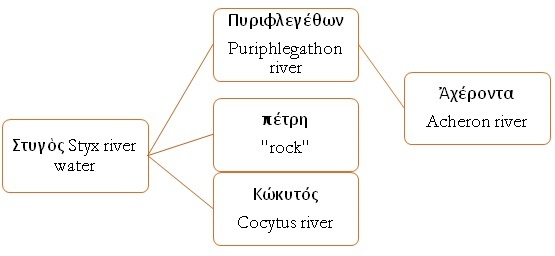
\includegraphics[width=\linewidth]{figures/Norman_figure1}%<<-- the relative-path of the figure --> it is stored in the folder "figures" and its filename is "testfigure"
			\caption{Geographical diagram}
			\label{normann_figure1} %best is to use the name of the file
		\end{figure}
\noindent Based on this passage, a geographical diagram can be drawn (fig. \ref{normann_figure1}).
Gurney suggests that honey, one of the offerings mentioned, was used in the village north of the Cappadox river (Delije Irmak) \parencite[77]{Gurney1990}. In the north of the Cappadox there are two rivers surrounding a small main land covered by rocks. This resembles the description Homer gives, indicating it may have been the area of the Cimmerians. Hoffner translated a Hittite text that declares honey was also offered by a rock \parencite[346]{Hoffner1997}, this bears a strong resemblance to Homer, at the \emph{petre} “rock” in the underworld, offering honey to the dead. The Hittite law code contains the offerings that Homer mentions: wine, bull, sheep, and barley \parencite[82]{Gurney1990}. This list of agricultural produce, particularly honey, was well known in the north of Cappadox and valued as one shekel. It would seem that the higher the price, the larger the demand. Thus, the honey might have been in high demand for the rituals it was used to perform. The produce mentioned in the law code were the same as those offered by Odysseus. This similarity between the two locations and their offerings might indicate further the underworld was in Cappadox. Rocks, \emph{hekur}, were considered sanctuaries \parencite{Slocum2014}, associated with the funerary cult of dead kings \parencite[43]{Harmansah2014}. Homer’s description of the rock, being the meeting place of the deceased, would be considered a funerary sanctuary for the dead. The similarities between the rock as meeting place for the dead in Homer’s underworld and the rock as a funerary sanctuary in Hittite customs suggest that north of Cappadox was the general area of the underworld Homer describes. 
	
	The theory above, however, is based on only one of the possible translations of \emph{petre}. Though translated as a “rock” \parencite{Liddell1940}, the term is also used to describe rocks as cliffs by the sea. The earliest mention of this is in Homer’s \emph{Odyssey}, Book III, “A smooth rock is high and steep to the sea, to the furthest of Gortuna in the misty and cloudy dark sea.” (author’s translation, Hom.Od.3.293–4). This association of \emph{petre} with cliffs was known, and perhaps implied, in later translations. This suggestion can be applied to the description of the Cimmerians: “We first dragged the ship to steep heaven [sky]” (author’s translation, Hom. Od.11.2). Despite the differences between the steep rock and sky, they both seem to share the same attributes. Possibly the same place is being described. It could be the concept of a high steep rock is similar to the mountain. Mount Olympus is associated with the presence of the sky (heaven), when Ares comes and visits the resting place of the gods (Hom. Il. 5.866 –8). It may suggest that Homer’s description of the protagonist and sailors going to the steepest sky is a hyperbolic description of the mountain or cliffs in Cimmeria. The similar descriptions of these steep rocks in Books III and XI may then suggest that the same location is being described. If true, Egypt could be a possible location as the Papyrus of Ani describes the \emph{3ht} mountain cliffs as the meeting place for the spirits of life and resurrection in the same way Odysseus goes to the cliffs to resurrect the dead spirits to life. Nonetheless, to be certain, this does require more evidence and wider analysis of both texts.
	
	In Book XI, Odysseus and the sailors come to the land of the Cimmerians, whose sun never reaches the stars (Hom.Od.11.15–18). They were people covered in clouds (νεφέλῃ). This description is not different from the one Homer gives of the \emph{eroeidei pontoi}, “the cloudy dark sea” in Gortuna Crete. The same environmental features of both locations suggest the same area might have been described, the lower part of the Mediterranean (near Crete). This would suggest Egypt, being by the southern Mediterranean, might have been a possible location. The Egyptians, in the Papyrus of Ani, show a sun descending between two cliffs (\emph{3ht}) when the \emph{‘anh} (life) ibis bird and the phoenix bird (resurrection) are present. The \emph{3ht} is shown twice. The first one is a darker image of the sun, a suggestion it represents sunset. The other, below, shows a much lighter sun, indicating sun rise. The lack of its full appearance indicates they are in a persistent state of semi darkness. This is no different from the description Homer gives: that the sun, which shines with rays would never go to star filled heaven, nor does it ever urge itself towards the land (Hom. Od. 11.16–17), indicating a persistent sun rise and sun set. The details Circes provides of the \emph{petre} steep rock, being in between the two rivers does also seem to be a concept shown in the Papyrus of Ani, where the land on the second island is surrounded by two rivers of water, and two cliffs which surround the sun. The similar geographical descriptions of these areas, might indicate the same area is being described, suggesting that the location of the Homeric underworld resides in Egypt.
	
	
%	\section{Geography of the Underworld: Location of Oceanus}
	
	
	Further\marginnote{Geography of the Underworld: Location of Oceanus} consideration of the geographical descriptions might add more to our understanding of the location of the underworld. Homer describes the area of Cimmeria as being in the realm of the deep Oceanus \emph{bathurouu Okeanoio} (Hom.Od.11.13) The deep nature of Oceanus give an indication an ocean itself is being described. Homer gives a profound description of this mythological body of water in the \emph{Iliad}: “The great strength of deep Oceanus, out of which all rivers and every sea and all springs and wells flow” (author’s translation, Hom.Il. 21.195–7). Thereby giving the impression that Homer was describing an area of the Ocean surrounded by rivers. Geographically, this resembles the lower area of the Mediterranean, close to Asia Minor and Egypt, the Delta Nile. This theory is considered later by Diodorus Siculus, who states the name \emph{Okeaen}, called by the Greeks Oceanus, referred to the rivers of Egypt (Diod. 1.19). This might indicate Oceanus was in the Mediterranean Sea and would allow us to consider the entrance of the underworld to be in Egypt. 
		
	Though it has to be queried why, in Homer’s poetry, Oceanus would be in the Mediterranean and not in any other alluvial plain. Mackie’s doubts of whether the chthonic rivers themselves were a part of the Cimmerian location are justified. His discussion of Oceanus as an encircling river raises the question whether Acheron, Cocytus, Styx, or Puriphlegathon rivers were in the same location \parencite[486]{Mackie1999}. Homer describes Oceanus as a \emph{potamoio} “river” (Hom.Od.12.1) rather than the Mediterranean Ocean. However, it has already been acknowledged that Homer was in close contact with the Phoenicians and Assyrians. The Babylonians and Assyrians, much like Homer’s Oceanus, saw their world as encircled by a river (ME 92687). This river shown on the clay tablet was created in 700 \BC, theoretically the same time as Homer. The profound similarity between Homer’s Oceanus and this Assyrian-Babylonian map of the world, can only suggest Homer was inspired by the Assyrian and Babylonian beliefs and myths. If true, then it is also likely their writing influenced him. West demonstrated that the Assyrian word for river was (the same word in the Babylonian map of the world) also used in the seventh century BC to describe the Mediterranean \parencite[145]{West1997}. That being the case, Homer, having this myth passed down to him by the Assyrians, could have viewed the river of Oceanus in the same way, as a representation of the eastern Mediterranean.
		
	Given the importance of the Phoenicians’ influence in Homer’s writing, it is also important to consider whether the river of Oceanus was seen to represent the Mediterranean. In the Levant the closest Semitic group to the coast would have been the Aramaic Canaanites. Their inhabitance in a coastal area, would have mean they were able to create sea trading posts and be, in Greek thought, associated with the Phoenicians. There is a possibility the Greek word \emph{potamoi} derived from the two Aramaic words \emph{P-THh} “open” \parencite[422]{Benner2005} and \emph{MH} “sea” \parencite[166]{Benner2005}. Combined, these two read \emph{pthhmh} (\emph{potehhmah}), “Open sea”. This would indicate Homer saw \emph{potamoio Okeanoio} not as a chthonic river, but rather a chthonic Ocean. The \emph{PTHh}, according to \textcite{Benner2005}, represents a subject breaking away from something else. \emph{Mh}, on the other hand, was said to refer to the Mediterranean and feared by the Semitic groups for its deep nature. Homer describes the \emph{potamoi} Oceanus, much like the Semitic Mediterranean, as deep and feared as their limits were where the dead reside. This would indicate the Mediterranean and Oceanus were the same.  In Homeric thought, however, the term \emph{Okeanoio} potamoio might have been a colloquial, shortened title, from the description Homer gives in the Iliad:
	
	\begin{quote}
		
	“βαθυρρειταο μεγα σθενος Ωκεανοιο,
	εξ ου περ΄παντες ποταμοι και πασα θαλασσα,
	και πασαι κρηναι και φρειατα μαχρα ναουσιν:” (Hom. Il. 21.196).
		
	“The great strength of deep Oceanus, out of which every river, every sea and every fountain and artificial well flows.” (Author’s translation).
	
	\end{quote}
To Homer the rivers flow from deep Oceanus, indicating it is a far larger source of water, an ocean. This would suggest that the description of \emph{potamoio Okeano} does not describe Oceanus as a river, but rather is a title to describe that which flows out from it, the rivers. It is reasonable to suggest that Oceanus, for its deep nature, is an Ocean. It is also important to take notice of the fact that every river flows from Oceanus. This would give the indication that it is in an area that is attached to a series of rivers. The Mediterranean resembles this description in that the rivers of the Delta Nile flow from this particular ocean. This indicates Oceanus was describing the Mediterranean closest to the Delta Nile and Egypt. As Oceanus is the body of water, representing the Mediterranean, that leads to the rivers of the underworld, it could be argued that these rivers represents the delta Nile, giving more reason to believe the underworld was located in Egypt. 
		
	The similar environmental features in the locations described in both the Book of the Dead and Homeric Underworld might also indicate the same area is being described by these two documents. Given that the Egyptian Book of the Dead predates the poet, it is possible that Homer was influenced by this document and would associate the location mentioned in the funerary texts with Egypt. An example of this Egyptian influence of the Homeric underworld would be the Papyrus of Ani (EA10470/35). The Papyrus shows Ani (the deceased) in the Field of Offerings when the sun is eclipsed, making offerings of agricultural work to the gods and Osiris, and there are some similarities with this and the \emph{Odyssey}. 
	
	\begin{quote}
		
	‘oυδε ποτ’ αυτους, 
	ηελιος φαεθων καταδερχεται αχτινεσσιν, 
	ουθ’ οποτ’ αν στειχησι προς ουρανον αστεροεντα’ (Hom.Od.11.15–18).
		
	“Never does the sun, shining with rays, look down on them, neither would it come to star-filled heaven.” (Author’s translation).
	
	\end{quote}
		The Papyrus of Ani shows similar details. In the first passage, the sun is eclipsed, matching the description that the place of the underworld is filled with darkness. Such similar environmental features between these two areas would indicate the same area is being described. Given that the Book of the Dead predates Homer, it is possible the poet was inspired by this aspect of Egyptian mythology, and from this might have considered to position the Greek underworld in Egypt.  
	
	
%	\section{Ritual and Offerings to Gods: Homeric and Egyptian}
	
	
	There\marginnote{Ritual and Offerings to Gods: Homeric and Egyptian} is one flaw in presuming the underworld is set in Egypt. Circes mentions that the north wind should take Odysseus to the underworld (Hom. Od.10.507). An argument could be put forward that the underworld is set north. This, though, may be too quick a judgment to make. One interpretation, when looking at Hesiodic sources, is that the north wind, Boreas, blows southward from the north. Hesiod describes Boreas’ movements in some detail:
	
	\begin{quote}
	
	“και πηγαδας, αιτ’ επι γαιαν, πγευσαντος Βορεαο δυσηλεγεες τελεθουσιν,
	οστε δια Θρηικης ιπποτροφου ευρει ποντωι,
	εμπνευσας ωρινε’  (Hes.WD. 505-508).
	
	“…and frosts, which are cruel come into being, while Boreas having blown towards the land and having blown through horse-bred Thrace to the wide sea, stirs it up.” (Author’s translation).
	
	\end{quote}
	
	Thrace, what is now largely considered Bulgaria, was an area north of Greece. Hesiod makes a point of mentioning that Boreas blows through this area \emph{dia Threikes}, to the wide sea, \emph{eurei pontoi}. From Hesiod’s perspective, as a Boeotian, the widest noticeable sea would have been the Aegean or Mediterranean (south of Thrace). This does give reason to think that Boreas blows from Thrace (north of Boeotia) to an ocean south from this area. Given that Homer was debatably alive at the same time as Hesiod, and theoretically from a close location, Euboea, it is possible he also believed Boreas to have come from the north and blown southwards. Evidence of this can be seen in the \emph{Odyssey}, when the poet uses the compound verb \emph{katelthomen} “we went down” (Hom.Od.11.1), referring to Odysseus and the sailors going down from the Aegean to the underworld. This would imply they were going southward, and that the underworld by extension was south of them. If true then the north wind Boreas would blow them from Aegeus to a southern direction, which might have been the Mediterranean Sea. This would give reason to think that, as the Mediterranean is south of Aegeus, so is the underworld, indicating they may have been the same location to Homer. That said though the Mediterranean encompasses Asia Minor, the Levant and Egypt. This would not therefore show the specific location of the underworld, which means further analysis is needed.
	
	Another interpretation is that the Homeric north wind was inspired by the Egyptian underworld. In the Book of the Dead it is the wind that carries the traveller from \emph{Tem} to \emph{Khent Amenti} \parencite[300]{Budge1969}. The similarities between the two winds taking the traveller to the underworld, might indicate Homer was inspired by the Book of the Dead. If true, Homer might well have intended to set the underworld in Egypt, because of their mythology’s influential nature. A suggestion could also be made that the Cimmerians were, in fact, the domain of \emph{Khenti Amenti}. The title \emph{Khent Amenti}, in the Papyrus of Nakht (EA 10471/21), has a determinative for a desert; often the burial place of the dead. This suggests \emph{Khenti Amenti} was a specific chthonic area in Egyptian mythology. The Papyrus of Nakht contains similar imagery as Cimmeria described by Circes in the \emph{Odyssey} Book X. She mentions that Cimmeria contains black poplars, which lose their fruit beside a pool of water (Hom. Od.10. 510). The Papyrus of Nakht appears to show this same description: long trees (much like poplars) surround a pool of water. One tree in particular, containing black fruit, dangles and falls towards Osiris. The striking similarity between these two areas could mean that the same area is being described. This, and the presence of the north wind, in Egyptian mythology, indicates Homer’s underworld was located in Egypt.
	
	Throughout Book XI there is no mention of the offerings being dedicated to Hades. This is considerably different from the Book of the Dead cxxxviia that mentions the offerings were dedicated to the Lord of the Underworld, Osiris. This distinction between the two offerings would indicate Homer was not inspired by Egyptian rituals. Book X line 535, however, implicates the offerings were made to Hades, Lord of the Underworld: “to make prayers for the gods and to strong Hades and to pray for Persephone” (Hom.Od.10.533–4).The emphasis of the prayers made to Hades would suggest the offerings were dedicated to him, much like they were to Osiris. This, though it tells us little about whether the Book of the Dead was an inspiration, does encourage us to look further and see if there is more conclusive evidence to suggest the underworld was in Egypt.
	
	There is a conundrum (presuming the location is, in vague terms, an area set within Egypt) about whom the offerings are made; to the sun god Ra or the Lord of the Underworld Osiris. In the same way, it is difficult to say exactly which offerings were made to the gods of the underworld in Greek culture; whether it was Helios or Hades. Homer, as mentioned before, does not clearly specify at the beginning of Book XI whether any of these offerings were made to any Greek deities in particular. He does, however, give clear descriptions of the offerings themselves. He places particular emphasis on the sacrificing of a “black ram” (Hom.Od.11.32–33) an important description since similar offerings are shown in Egyptian culture. Named by the Manchester Museum as the “Stelae of Penwimetreru” (Acc. no. TN R4571/1937), this particular \emph{stelae} shows ram funeral offerings made to Amun Ra, lord of the sky. As opposed to other \emph{stelai} of the new kingdom, however, there is no mention in the first column of what the offerings themselves are, although, above the hieroglyphic inscriptions, there are two large rams inscribed as \emph{imn ra}, Amun Ra.
	
	Given that these animals are the most noticeable features of the \emph{stelae}, it is possible the offerings are the rams mentioned above. Suggesting that Homer, based on these similar offerings, intended the rams to be given as a sacrifice to the sun god Helios (in the same way they were given to the sun god Amun Ra). Helios, however, in both Books X and XI of the \emph{Odyssey}, seems to be used only evocatively. That is to say the sun is only treated as a feature of the environment, not a deity. As has been previously discussed, Homer does mention that prayers were made to Hades, which could imply the sacrifices were offered to him as well. This observation would give the impression that offerings were made to Hades himself rather than to Helios. A suggestion can therefore be put forward that Hades worship was inspired by the worship made to Osiris. Such influences, though not specific enough on their own to prove the location, can encourage us to further analyse the role of Osiris and whether there is any connection between his and Hades’ offerings that could indicate the underworld resides in Egypt.
	
	The distinct offerings of rams to Hades, as Homer describes, could have been inspired by the ram-like nature of Osiris, Lord of the Underworld. Before inspecting the Homeric poetry in Book XI, it is important to pay attention to Egyptian influences on Homer underworld. The tomb of Prince Mentuherkhepsef shows a ram-headed deity, known as \emph{Banebdedjet}, holding a scepter shaped to resemble the \emph{Djed} and \emph{ankh} symbol. He is given offerings of oils and incense. To the right of the image is an inscription written in hieroglyphic form \emph{ba-nb-dd-dd}. (KV.19.NO.19). While this has simply been labeled as a name of the deity, the title could well have been an epithet for Osiris. Gardiner says; “\emph{Ba} meant the modes of existence with which the deceased continued to live” \parencite[15]{Zabakar1968}, indicating ba enabled the dead to live. Homer shows a similar concept, by Odysseus seeing the \emph{psuches} “lives” of the deceased in Book XI. The \emph{ba} sign, however, is represented as a ram. This could be allegorical, representing both a soul and offering of a ram, similar to the ram Homer describes. While the \emph{ba} ram could be translated as an aspect of the soul, some scholars state the animal symbolising the \emph{ba} soul is the \emph{jabiru} \parencite[107]{Betro1996}. It could be that the meaning behind the \emph{ba} ram is a determinative, a symbol of what was offered. This could translate to mean: “the ram for the \emph{ba} of the lord of \emph{dddd}”, thereby similar to the offering Homer gives of the ram itself. Just below this and the two \emph{dd} symbols is a determinative, \emph{niwt}, the determinative of a city or region \parencite[190]{Betro1996}, implying \emph{dd} refers to a place. Given the observation of each hieroglyph, it is unwise to label this simply as a name for the god, but rather a description of who he represents “the existing soul of the lord of the region \emph{dddd}”. In the funeral \emph{stelai} of the New Kingdom (specifically the eighteenth dynasty), the Stelae of Senres and Hormose (Acc. No. 07,420), Osiris is known as the lord of \emph{DDW} region. 
	
	Another \emph{stelae}, belonging to the New Kingdom (A.No.22.155), shows the name of the region \emph{ddw} written as \emph{ddddw}. The display of two \emph{djed} symbols in this \emph{stela} shows the location of \emph{DDW}. The quail (\emph{w}) bird is absent in KV.19 No.19 art, however the similarities to the writing of \emph{ddw} are noticeable. This gives the implication the area described in the title \emph{Ba-nb-dd}, is \emph{ddw} itself. Therefore the \emph{ba-nb-dddd} could describe “the constant existing soul of the lord of \emph{ddw}” which would be Osiris. This translation of offering a ram to Osiris resembles the offering of a ram to Hades which Homer gives to Teireses (Hom.Od.XI,32). This would suggest Homer’s offerings were inspired by Egyptian rituals, reinforcing the idea that the Underworld location is in Egypt. 
	
	Furthermore, the above passage bears similarities to the Book of the Dead. Homer mentions that the sun never reaches heaven where the stars reside. This implies that the stars are never known to set. Such a feature of the Underworld is seen in chapter XCVIII of the Book of the Dead: “And the stars which never rest set [me] away from the slaughter” \parencite[296]{Budge1969}. The mention of the stars keeping the subject away from slaughter indicates he is a living mortal. Homer makes no mention of Odysseus’ death and is presumed living, much like the figure in the Book of the Dead. This similarity would indicate that Homer was inspired by the Book of the Dead. Further evidence supports this theory: the Papyrus of Nu (EA. 10/477 Sheet 21–22), found in Budges translation, displays a man in a boat. Just below where he is stationed is the symbol \emph{udjat}, the eye of Horus. The \emph{udjat} itself symbolises healing, a suggestion the person was protected from death, and therefore alive. This is similar to Odysseus being alive while visiting the Underworld. The same concept was used by Homer therefore supposes there was a shared belief system between Homeric mythology and Egyptian. This further propounds that the location of the Homeric underworld was in Egypt. 
	
	
%	\section{Conclusion}
	
	
	In\marginnote{Conclusion} conclusion, more evidence indicates that the mythical Cimmerians were part of the Egyptian territory. While there are certain similarities between Homeric and Hittite rituals, the offerings Homer describes as well as their purpose correspond strongly with the Egyptian belief system in the New Kingdom, in resurrecting the deceased. Not only this but the geographical descriptions Homer provides from Books X–XII are similar to the descriptions provided in the Papyrus of Ani, Nu and Nahkt. The parallels between the Homeric and Egyptian geographical and ritual description, prove that Egypt might have been the location Homer described. 
	
	
%	\section{Assessment}
	
	
	The\marginnote{Assessment} purpose of this article was to gain a general understanding of the location of the Homeric Underworld.  The process of research has shown there to be a possibility the underworld was located within Egypt. Although the comparison between Homeric, Egyptian and Anatolian offerings helped to gain a broader understanding of the location, the results were not as conclusive as would have been expected. The offerings described by Homer in the \emph{Odyssey} Book X and XI were similar to Hittite and Egyptian rituals, which, on its own, did not give enough conclusive evidence to mark a particular location. Nevertheless the ritual evidence, coupled with the inspection of Homer’s geographical descriptions, both helped to narrow the analysis further. The ability to look at parallels between Homeric Cimmerian rituals and geographical details with Egyptian, helped to conclude the Homeric Cimmerians were set in Egypt.
	
	While the evidence presented should help readers to assess the location of the Cimmerian underworld differently, I would encourage scholars to investigate Babylonian influences further. For example, compare the Homeric description of the chthonic rivers, and Oceanus, with Nineveh and the Babylonian map of the world further (ME 92687) and see if the Homeric Oceanus was located in Mesopotamia or the Mediterranean. In addition, while this article has focused on Ugaritic etymology, the derivation of the word \emph{potamoi}, I would strongly recommend investigating Akkadian writings, and see how influential they were on Homer’s location of the Cimmerian underworld. 
\myseparator	
%	\section{Acknowledgements}
I would\marginnote{Acknowledgements} like to take this opportunity to thank my friends and family for their support during the writing of this article. Their feedback has been of great value, and one of the reasons I have persevered with this research. I would particularly like to thank Dr. Rosie Wyles and Dr. Kellie Rudolph for their willingness to review the research conducted at the early stages of the article. Both highly regarded scholars, their professional assessment of the research and overall structure of the piece helped me to develop further investigations into the location of the Homeric Underworld.
			
			

\begin{myabstract}
	\foreignlanguage{ngerman}{%
		Die Homerischen Epen zeigten die ersten grundlegenden Strukturen der griechischen Unterwelt auf: der die Welt umfließende tiefe Strom Okeanus, die Flüsse Styx, Acheron Cocytus, und das feuchtkalte „Haus des Hades“. Ziel dieses Artikels ist, ein allgemeines Verständnis davon zu bekommen, wo die homerische Unterwelt lokalisiert war, insbesondere die Unterwelt im elften Buch der \emph{Odyssee}. 
		Um den genauen Ort zu bestimmen, benutzt der Artikel eine Kombination aus archäologischen Befunden, vergleichenden sprachwissenschaftlichen Untersuchungen hethitischer und ägyptischer \emph{stelai} und \emph{papyri}, sowie eine Literaturanalyse der homerischen Epen.}
	
	\keywords[Schlüssbegriffe]{Homer, Mythologische Geographie, Odyssee, Hethiter, Unterwelt, Buch der Toten, Kimmerer, Bronzezeit Mittelmeer.}
\end{myabstract}

	
	
\printbibliography[heading=subbibnumbered] 
\label{Norman:lastpage}
\closingarticle
